%%%%%%%%%%%%%%%%%
% Configuration %
%%%%%%%%%%%%%%%%%

\documentclass[12pt, a4paper, twocolumn]{article}
\usepackage{amsmath}
\usepackage{amssymb}
\usepackage{mathtools}
\usepackage{csquotes}
\usepackage{xurl}
\urlstyle{rm}
\usepackage[super,comma,sort]{natbib}
\bibliographystyle{plainnat}
\usepackage{abstract}
\renewcommand{\abstractnamefont}{\normalfont\bfseries}
\renewcommand{\abstracttextfont}{\normalfont\itshape}
\usepackage{lipsum}
\usepackage{booktabs}
\usepackage{geometry}
\geometry{top=1cm,bottom=1.5cm,left=2cm,right=2cm,includehead,includefoot}
\setlength{\columnsep}{7mm} % Column separation width
\renewcommand*{\thefootnote}{\roman{footnote}}
\renewcommand*{\bibfont}{\raggedright}
\usepackage{float}
\usepackage{graphicx}
\usepackage{subcaption}
\usepackage{bm}
\raggedbottom
\usepackage[bottom]{footmisc}
\interfootnotelinepenalty=100 % Default 100, increase to reduce footnote splitting.
\newcommand\nothing{}

% Inline equations: https://tex.stackexchange.com/a/78582/178803
\makeatletter
\newcommand*{\inlineequation}[2][]{%
  \begingroup
    % Put \refstepcounter at the beginning, because
    % package `hyperref' sets the anchor here.
    \refstepcounter{equation}%
    \ifx\\#1\\%
    \else
      \label{#1}%
    \fi
    % prevent line breaks inside equation
    \relpenalty=10000 %
    \binoppenalty=10000 %
    \ensuremath{%
      % \displaystyle % larger fractions, ...
      #2%
    }%
    ~\@eqnnum
  \endgroup
}
\makeatother

%%%%%%%%%%%%%%
% References %
%%%%%%%%%%%%%%

\begin{filecontents}{value_based_prioritization.bib}

@InCollection{scientific-method,
  author       = {Andersen, Hanne and Hepburn, Brian},
  title        = {Scientific Method},
  booktitle    = {The Stanford Encyclopedia of Philosophy},
  editor       = {Edward N. Zalta},
  note         = {\url{https://plato.stanford.edu/archives/sum2016/entries/scientific-method/}},
  year         = {2016},
  edition      = {Summer 2016},
  publisher    = {Metaphysics Research Lab, Stanford University},
}

@article{martela2016three,
  title        = {The three meanings of meaning in life: Distinguishing coherence, purpose, and significance},
  author       = {Martela, Frank and Steger, Michael F},
  journal      = {The Journal of Positive Psychology},
  volume       = {11},
  number       = {5},
  pages        = {531--545},
  year         = {2016},
  publisher    = {Taylor \& Francis},
  note         = {\url{https://www.ippanetwork.org/wp-content/uploads/2017/02/Martela-Steger-JOPP.pdf}},
}

@book{huemer2007ethical,
  title        = {Ethical Intuitionism},
  author       = {Huemer, Michael},
  year         = {2007},
  publisher    = {Springer},
  note         = {\url{https://spot.colorado.edu/~huemer/5.htm}},
}

@book{huemer2013problem,
  title        = {The Problem of Political Authority},
  author       = {Huemer, Michael},
  year         = {2013},
  publisher    = {Springer},
  note         = {\url{https://spot.colorado.edu/~huemer/1.htm}},
}

@InCollection{value-theory,
  author       = {Schroeder, Mark},
  title        = {Value Theory},
  booktitle    = {The Stanford Encyclopedia of Philosophy},
  editor       = {Edward N. Zalta},
  note         = {\url{https://plato.stanford.edu/archives/fall2016/entries/value-theory/}},
  year         = {2016},
  edition      = {Fall 2016},
  publisher    = {Metaphysics Research Lab, Stanford University},
}

@InCollection{consequentialism,
  author       = {Sinnott-Armstrong, Walter},
  title        = {Consequentialism},
  booktitle    = {The Stanford Encyclopedia of Philosophy},
  editor       = {Edward N. Zalta},
  note         = {\url{https://plato.stanford.edu/archives/win2015/entries/consequentialism/}},
  year         = {2015},
  edition      = {Winter 2015},
  publisher    = {Metaphysics Research Lab, Stanford University},
}

@InCollection{ayn-rand,
  author       = {Badhwar, Neera K. and Long, Roderick T.},
  title        = {Ayn Rand},
  booktitle    = {The Stanford Encyclopedia of Philosophy},
  editor       = {Edward N. Zalta},
  note         = {\url{https://plato.stanford.edu/archives/fall2017/entries/ayn-rand/}},
  year         = {2017},
  edition      = {Fall 2017},
  publisher    = {Metaphysics Research Lab, Stanford University},
}

@InCollection{religion-morality,
  author       = {Hare, John},
  title        = {Religion and Morality},
  booktitle    = {The Stanford Encyclopedia of Philosophy},
  editor       = {Edward N. Zalta},
  note         = {\url{https://plato.stanford.edu/archives/win2014/entries/religion-morality/}},
  year         = {2014},
  edition      = {Winter 2014},
  publisher    = {Metaphysics Research Lab, Stanford University},
}

@InCollection{morality-biology,
  author       = {FitzPatrick, William},
  title        = {Morality and Evolutionary Biology},
  booktitle    = {The Stanford Encyclopedia of Philosophy},
  editor       = {Edward N. Zalta},
  note         = {\url{https://plato.stanford.edu/archives/spr2016/entries/morality-biology/}},
  year         = {2016},
  edition      = {Spring 2016},
  publisher    = {Metaphysics Research Lab, Stanford University},
}

@InCollection{epicurus,
  author       = {Konstan, David},
  title        = {Epicurus},
  booktitle    = {The Stanford Encyclopedia of Philosophy},
  editor       = {Edward N. Zalta},
  note         = {\url{https://plato.stanford.edu/archives/sum2018/entries/epicurus/}},
  year         = {2018},
  edition      = {Summer 2018},
  publisher    = {Metaphysics Research Lab, Stanford University},
}

@InCollection{stoicism,
  author       = {Baltzly, Dirk},
  title        = {Stoicism},
  booktitle    = {The Stanford Encyclopedia of Philosophy},
  editor       = {Edward N. Zalta},
  note         = {\url{https://plato.stanford.edu/archives/sum2018/entries/stoicism/}},
  year         = {2018},
  edition      = {Summer 2018},
  publisher    = {Metaphysics Research Lab, Stanford University},
}

@InCollection{rawls,
  author       = {Wenar, Leif},
  title        = {John Rawls},
  booktitle    = {The Stanford Encyclopedia of Philosophy},
  editor       = {Edward N. Zalta},
  note         = {\url{https://plato.stanford.edu/archives/spr2017/entries/rawls/}},
  year         = {2017},
  edition      = {Spring 2017},
  publisher    = {Metaphysics Research Lab, Stanford University},
}

@InCollection{communitarianism,
  author       = {Bell, Daniel},
  title        = {Communitarianism},
  booktitle    = {The Stanford Encyclopedia of Philosophy},
  editor       = {Edward N. Zalta},
  note         = {\url{https://plato.stanford.edu/archives/sum2016/entries/communitarianism/}},
  year         = {2016},
  edition      = {Summer 2016},
  publisher    = {Metaphysics Research Lab, Stanford University},
}

@article{weinstein2009qalys,
  title        = {{QALYs: the basics}},
  author       = {Weinstein, Milton C and Torrance, George and McGuire, Alistair},
  journal      = {Value in health},
  volume       = {12},
  pages        = {S5--S9},
  year         = {2009},
  publisher    = {Wiley Online Library},
  note         = {\url{https://onlinelibrary.wiley.com/doi/pdf/10.1111/j.1524-4733.2009.00515.x}},
}

@article{wit2012all,
  title        = {‘All models are wrong...’: an introduction to model uncertainty},
  author       = {Wit, Ernst and Heuvel, Edwin van den and Romeijn, Jan-Willem},
  journal      = {Statistica Neerlandica},
  volume       = {66},
  number       = {3},
  pages        = {217--236},
  year         = {2012},
  publisher    = {Wiley Online Library},
  note         = {\url{https://www.rug.nl/research/portal/files/13270992/2012StatistNeerlWit.pdf}},
}

@misc{centers2017underlying,
  title        = {{Underlying Cause of Death 1999-2017 on CDC WONDER Online Database, released December, 2018. Data are from the Multiple Cause of Death Files, 1999-2017, as compiled from data provided by the 57 vital statistics jurisdictions through the Vital Statistics Cooperative Program}},
  author       = {{Centers for Disease Control and Prevention and National Center for Health Statistics}},
  howpublished = {\url{https://wonder.cdc.gov/ucd-icd10.html}},
  note         = {Accessed: 2019-03-01},
}

@book{icd10vol1,
  title        = {International statistical classification of diseases and related health problems},
  author       = {World Health Organization},
  year         = {2016},
  publisher    = {World Health Organization},
  edition      = {10th},
  volume       = {1},
  note         = {\url{https://apps.who.int/iris/bitstream/handle/10665/246208/9789241549165-V1-eng.pdf}},
}

@book{icd10vol2,
  title        = {International statistical classification of diseases and related health problems},
  author       = {World Health Organization},
  year         = {2010},
  publisher    = {World Health Organization},
  edition      = {10th},
  volume       = {2},
  note         = {\url{https://www.who.int/classifications/icd/ICD10Volume2_en_2010.pdf}},
}

@book{icd10vol3,
  title        = {International statistical classification of diseases and related health problems},
  author       = {World Health Organization},
  year         = {2016},
  publisher    = {World Health Organization},
  edition      = {10th},
  volume       = {3},
  note         = {\url{https://apps.who.int/iris/bitstream/handle/10665/246208/9789241549165-V3-eng.pdf}},
}

@article{anderson2004model,
  title        = {Model selection and multi-model inference},
  author       = {Anderson, DR and Burnham, K},
  journal      = {Second. NY: Springer-Verlag},
  year         = {2004},
}

@article{burnham2004multimodel,
  title        = {Multimodel inference: understanding AIC and BIC in model selection},
  author       = {Burnham, Kenneth P and Anderson, David R},
  journal      = {Sociological methods \& research},
  volume       = {33},
  number       = {2},
  pages        = {261--304},
  year         = {2004},
  publisher    = {Sage Publications Sage CA: Thousand Oaks, CA},
  doi          = {10.1177/0049124104268644},
  note         = {\url{http://www.sortie-nd.org/lme/Statistical\%20Papers/Burnham_and_Anderson_2004_Multimodel_Inference.pdf}},
}

@book{berk2004regression,
  title        = {Regression analysis: A constructive critique},
  author       = {Berk, Richard A},
  volume       = {11},
  year         = {2004},
  publisher    = {Sage},
}

@book{hyndman2018forecasting,
  title        = {Forecasting: principles and practice},
  author       = {Hyndman, Rob J and Athanasopoulos, George},
  year         = {2018},
  publisher    = {OTexts},
  note         = {\url{https://otexts.com/fpp2/}},
}

@article{clemen1989combining,
  title        = {Combining forecasts: A review and annotated bibliography},
  author       = {Clemen, Robert T},
  journal      = {International journal of forecasting},
  volume       = {5},
  number       = {4},
  pages        = {559--583},
  year         = {1989},
  publisher    = {Elsevier},
  note         = {\url{https://faculty.fuqua.duke.edu/\~clemen/bio/Published\%20Papers/13.CombiningReview-Clemen-IJOF-89.pdf}},
}

@article{taylor2018forecasting,
  title        = {Forecasting at scale},
  author       = {Taylor, Sean J and Letham, Benjamin},
  journal      = {The American Statistician},
  volume       = {72},
  number       = {1},
  pages        = {37--45},
  year         = {2018},
  publisher    = {Taylor \& Francis},
  note         = {\url{https://peerj.com/preprints/3190.pdf}},
}

@article{makridakis2018m4,
  title        = {The M4 Competition: Results, findings, conclusion and way forward},
  author       = {Makridakis, Spyros and Spiliotis, Evangelos and Assimakopoulos, Vassilios},
  journal      = {International Journal of Forecasting},
  volume       = {34},
  number       = {4},
  pages        = {802--808},
  year         = {2018},
  publisher    = {Elsevier},
  note         = {\url{https://www.researchgate.net/profile/Spyros_Makridakis/publication/325901666_The_M4_Competition_Results_findings_conclusion_and_way_forward/links/5b2c9aa4aca2720785d66b5e/The-M4-Competition-Results-findings-conclusion-and-way-forward.pdf}},
}

@misc{censusestimates19001999,
  title        = {{Historical National Population Estimates}},
  author       = {{U.S. Census Bureau}},
  howpublished = {\url{https://www2.census.gov/programs-surveys/popest/tables/1900-1980/national/totals/popclockest.txt}},
  note         = {Accessed: 2019-03-01},
}

@misc{worldbankopendata,
  title        = {{World Bank Open Data: United States SP.POP.TOTL}},
  author       = {{World Bank}},
  howpublished = {\url{http://api.worldbank.org/v2/en/country/USA?downloadformat=csv}},
  note         = {Accessed: 2019-03-01},
}

@misc{nbermortality,
  title        = {{Mortality Data: Vital Statistics NCHS' Multiple Cause of Death Data, 1959-2017}},
  author       = {{The National Bureau of Economic Research}},
  howpublished = {\url{https://www.nber.org/data/vital-statistics-mortality-data-multiple-cause-of-death.html}},
  note         = {Accessed: 2019-03-01},
}

@misc{icdcomparabilityratios,
  title        = {{A Guide to State Implementation of ICD-10 for Mortality; Part II: Applying Comparability Ratios}},
  author       = {{Centers for Disease Control and Prevention and National Center for Health Statistics\nothing}},
  howpublished = {\url{https://www.cdc.gov/nchs/data/statab/document-for-the-states.pdf}},
  note         = {Accessed: 2019-03-01},
}

@article{mathers2006projections,
  title        = {Projections of global mortality and burden of disease from 2002 to 2030},
  author       = {Mathers, Colin D and Loncar, Dejan},
  journal      = {PLoS medicine},
  volume       = {3},
  number       = {11},
  pages        = {e442},
  year         = {2006},
  publisher    = {Public Library of Science},
  note         = {\url{https://journals.plos.org/plosmedicine/article/file?id=10.1371/journal.pmed.0030442\&type=printable}},
}

@misc{uspopulation19002001,
  title        = {{United States Population by Age, Race, and Sex, 1900-90, and 1991-2001}},
  author       = {{Centers for Disease Control and Prevention and National Center for Health Statistics\nothing\nothing}},
  howpublished = {\url{https://www.cdc.gov/nchs/nvss/mortality/historical_population.htm}},
  note         = {Accessed: 2019-03-01},
}

@misc{uslcod19001998,
  title        = {{Leading Causes of Death, 1900-1998}},
  author       = {{Centers for Disease Control and Prevention and National Center for Health Statistics\nothing\nothing\nothing}},
  howpublished = {\url{https://www.cdc.gov/nchs/nvss/mortality_historical_data.htm}},
  note         = {Accessed: 2019-03-01},
}

@book{lopez2006global,
  title        = {Global burden of disease and risk factors},
  author       = {Lopez, Alan D and Mathers, Colin D and Ezzati, Majid and Jamison, Dean T and Murray, Christopher JL},
  year         = {2006},
  publisher    = {The World Bank},
  note         = {\url{https://openknowledge.worldbank.org/bitstream/handle/10986/7039/364010PAPER0Gl101OFFICIAL0USE0ONLY1.pdf}},
}

@article{world2009guide,
  title        = {{WHO guide to identifying the economic consequences of disease and injury}},
  author       = {World Health Organization and others},
  year         = {2009},
  publisher    = {World Health Organization},
  note         = {\url{https://www.who.int/choice/publications/d_economic_impact_guide.pdf}},
}

@misc{givewellcosteffectiveness,
  title        = {{Some considerations against more investment in cost-effectiveness estimates}},
  author       = {{GiveWell.org}},
  howpublished = {\url{https://blog.givewell.org/2011/11/04/some-considerations-against-more-investment-in-cost-effectiveness-estimates/}},
  note         = {Accessed: 2019-03-01},
}

@book{jamison2017disease,
  title        = {Disease Control Priorities, (Volume 9): Improving Health and Reducing Poverty},
  author       = {Jamison, Dean T and Gelband, Hellen and Horton, Susan and Jha, Prabhat and Laxminarayan, Ramanan and Mock, Charles N and Nugent, Rachel},
  year         = {2017},
  publisher    = {The World Bank},
  note         = {\url{https://openknowledge.worldbank.org/bitstream/handle/10986/28877/9781464805271.pdf}},
}

@article{neumann2018comparing,
  title        = {Comparing the cost-per-QALYs gained and cost-per-DALYs averted literatures},
  author       = {Neumann, Peter J and Anderson, Jordan E and Panzer, Ari D and Pope, Elle F and D'Cruz, Brittany N and Kim, David D and Cohen, Joshua T},
  journal      = {Gates open research},
  volume       = {2},
  year         = {2018},
  publisher    = {Gates Foundation-Open Access},
  note         = {\url{https://dqo52087pnd5x.cloudfront.net/manuscripts/13870/5db9cb3d-9e5e-456b-9276-52dc2973b97b_12786_-_Peter_Neumann_V2.pdf}},
}

@article{bostrom2013existential,
  title        = {Existential risk prevention as global priority},
  author       = {Bostrom, Nick},
  journal      = {Global Policy},
  volume       = {4},
  number       = {1},
  pages        = {15--31},
  year         = {2013},
  publisher    = {Wiley Online Library},
  note         = {\url{http://www.existential-risk.org/concept.pdf}},
}

@book{macaskill2015doing,
  title        = {Doing good better: Effective altruism and a radical new way to make a difference},
  author       = {MacAskill, William},
  year         = {2015},
  publisher    = {Guardian Faber Publishing},
}

@misc{whomortality,
  title        = {{WHO Mortality Database}},
  author       = {{World Health Organization}},
  howpublished = {\url{https://www.who.int/healthinfo/statistics/mortality_rawdata/en/}},
  note         = {Accessed: 2019-03-01},
}

@article{de200625,
  title        = {25 years of time series forecasting},
  author       = {De Gooijer, Jan G and Hyndman, Rob J},
  journal      = {International journal of forecasting},
  volume       = {22},
  number       = {3},
  pages        = {443--473},
  year         = {2006},
  publisher    = {Elsevier},
  note         = {\url{http://www.est.uc3m.es/esp/nueva_docencia/comp_col_get/lade/tecnicas_prediccion/Practicas0708/Practica1/25\%20years\%20of\%20time\%20series\%20forecasting\%20(Gooijer\%20and\%20Hyndman).pdf}},
}

@misc{tashman1991automatic,
  title        = {{Automatic forecasting software: A survey and evaluation}},
  author       = {Tashman, Leonard J and Leach, Michael L},
  year         = {1991},
  publisher    = {Elsevier},
  note         = {\url{https://www.researchgate.net/profile/Len_Tashman/publication/223444048_Automatic_forecasting_software_A_survey_and_evaluation/links/5ad7af42aca272fdaf8029b3/Automatic-forecasting-software-A-survey-and-evaluation.pdf}},
}

@book{hyndman2008forecasting,
  title        = {Forecasting with exponential smoothing: the state space approach},
  author       = {Hyndman, Rob and Koehler, Anne B and Ord, J Keith and Snyder, Ralph D},
  year         = {2008},
  publisher    = {Springer Science \& Business Media},
  note         = {\url{http://www.exponentialsmoothing.net/}},
}

@InCollection{sep-rationalism-empiricism,
  author       = {Markie, Peter},
  title        = {Rationalism vs. Empiricism},
  booktitle    = {The Stanford Encyclopedia of Philosophy},
  editor       = {Edward N. Zalta},
  note         = {\url{https://plato.stanford.edu/archives/fall2017/entries/rationalism-empiricism/}},
  year         = {2017},
  edition      = {Fall 2017},
  publisher    = {Metaphysics Research Lab, Stanford University},
}

\end{filecontents}

\usepackage{hyperref}
\hypersetup{colorlinks=true, urlcolor=blue, linkcolor=blue, citecolor=blue}

\begin{document}

\title{Value-Based Prioritization\thanks{\url{https://github.com/freeradical13/ValueBasedPrioritization}}}

\author{Kevin Grigorenko\thanks{\href{mailto:kevin@myplaceonline.com}{kevin@myplaceonline.com}}}

\newcommand{\abstractText}{\noindent
A method is proposed to use value theory to quantitatively prioritize
potential actions to accomplish a goal. This method is applied to the
example of choosing meaningful work using an example value system based
on the desire to reduce suffering.
}

%%%%%%%%%%%%
% Abstract %
%%%%%%%%%%%%

\twocolumn[
  \begin{@twocolumnfalse}
    \maketitle
    \begin{abstract}
      \abstractText
      \newline
      \newline
    \end{abstract}
  \end{@twocolumnfalse}
]

\saythanks

%%%%%%%%%%%
% Article %
%%%%%%%%%%%

\section{Introduction}

Why should a particular goal be pursued (\enquote{Why})? Given a goal, what actions should be pursued to best accomplish said goal (\enquote{What})? Given an action, how should said action be pursued (\enquote{How})?

This article proposes that value theory usually best scopes \enquote{Why} and \enquote{What} and the scientific method usually best answers \enquote{How}. A method called Value-Based Prioritization is developed to answer the \enquote{What} question:

\begin{equation*}
  \begin{gathered}
    \textrm{Why: } \textit{Value Theory} \\
    \downarrow \\
    \textrm{What: } \textit{\textbf{Value-Based Prioritization}} \\
    \downarrow \\
    \textrm{How: } \textit{Scientific Method}
  \end{gathered}
\end{equation*}

\section{Why a Goal?}

\enquote{Why a Goal?} is usually best scoped using value systems because they are evaluative by nature\cite{value-theory}. Evaluating different value systems is left as an (lifelong) exercise for the reader\footnote{Example value systems include intuitionism\cite{huemer2007ethical}, consequentialism\cite{consequentialism}, evolutionary biology\cite{morality-biology}, religion\cite{religion-morality}, epicureanism\cite{epicurus}, stoicism\cite{stoicism}, political liberalism\cite{rawls}, anarcho-capitalism\cite{huemer2013problem}, communitarianism\cite{communitarianism}, objectivism\cite{ayn-rand}, etc.}.

\section{What Actions?}

\enquote{What Actions?} is usually best scoped by prioritizing actions because actions usually have differing effect sizes and time is limited. It follows from the value system used to answer \enquote{Why} that the same value system is used primarily to evaluate the priority of each action.

This article proposes a method called Value-Based Prioritization which builds a quantitative prioritization model based on predicted effect sizes. Raw prioritization scores are further scaled by contextual factors such as implementation time, cost, risk, and other judgments.

\section{How to do an Action?}

Given answers to \enquote{Why?} and \enquote{What?}, how to implement actions is usually best answered with the scientific method\cite{scientific-method,sep-rationalism-empiricism}: observations are made and rational thought is used to generate hypotheses, hypotheses are tested with experiments, and successful experiments lead to theories and results.

\section{Value-Based Prioritization}

A \textbf{value system} \inlineequation[value-system]{V} generates a \textbf{goal} \inlineequation[goal]{G(t)} (for some future time $t$) and a set of \textbf{mutually exclusive potential future actions} $A(t)$:

\begin{equation}\label{potential-actions}
  \begin{gathered}
    A(t) = \{A_1(t), \ldots, A_N(t)\}, \\
    N > 1
  \end{gathered}
\end{equation}

An action's \textbf{estimated relative accomplishment amount} $B(A(t))$ is an action's expected \textit{relative} (i.e. with respect to other actions) contribution towards accomplishing $G$(t):

\begin{equation}\label{action-amount}
  \begin{gathered}
    B(A(t)) = \mathbb{R}, \\
    0 \leq \mathbb{R} \leq 1
  \end{gathered}
\end{equation}

Thus, $G(t)$ is fully accomplished if all actions are accomplished:

\begin{equation}\label{goal-accomplished}
  G(t) = \sum_{i=1}^{N} B(A_i(t)) = 1
\end{equation}

A \textbf{value-based prioritization score} $C(A(t))$ is the result of the product of a set of \textbf{value-based prioritization scale functions} \inlineequation[scale-functions]{S = \{S_1, \ldots, S_N\}} multiplied by \eqref{action-amount}:

\begin{equation}\label{prioritization-score}
  \begin{gathered}
    C(A(t)) = B(A(t)) \cdot \prod_{j=1}^{N} S_j(A(t)), \\
    0 \leq S_j(B(A(t))) \leq 1
  \end{gathered}
\end{equation}

Example scale functions include implementation time, cost, risk, and other judgments. Ideally, scale functions should be defined before running the model to reduce bias. The set $S$ always includes the element $S_1(A(t)) = 1$. Note that $\sum_{i=1}^{N} C(A_i(t)) \neq G$ if any $S_j(A_i(t)) < 1$.

A \textbf{value-based prioritization} $Z(t)$ is a sequence of actions ordered by prioritization score \eqref{prioritization-score} in descending order:

\begin{equation}\label{vbp}
  \begin{gathered}
    Z(t) = (A_1(t), \ldots, A_N(t)), \\
    C(A_1(t)) \geq \ldots \geq C(A_N(t))
  \end{gathered}
\end{equation}

The first $k$ actions in $Z(t)$ should be executed in descending priority/proportion where \inlineequation[how-many-actions]{k} is chosen based on factors such as available concurrency, time, resources, etc.

\section{Modeled Value-Based Prioritization}

Historical data may be used to predict actions' estimated relative accomplishment amounts \eqref{action-amount} at a future time \inlineequation[modeled-future-time]{t_F}.

If each action has historical data $D(A)$:

\begin{equation}\label{action-predictors}
  \begin{multlined}
    D(A) = \\
    \shoveleft[0.5cm]{((t_1, D(A,t_1)), \ldots, (t_N, D(A,t_N)))}
  \end{multlined}
\end{equation}

Then, a set of \textbf{comparable prediction models} $R(D(A))$ is applied to each $D(A)$ (e.g. exponential smoothing\cite{hyndman2018forecasting,hyndman2008forecasting}\textsuperscript{,}\footnote{\scriptsize{\url{https://otexts.com/fpp2/expsmooth.html}}}, a generalized additive model [GAM]\cite{taylor2018forecasting}, ARIMA\cite{hyndman2018forecasting}\textsuperscript{,}\footnote{\scriptsize{\url{https://otexts.com/fpp2/arima.html}}}, linear regression\cite{hyndman2018forecasting}\textsuperscript{,}\footnote{\scriptsize{\url{https://otexts.com/fpp2/regression.html}}}, machine learning\cite{makridakis2018m4}, seasonal algorithms such as TBATS\cite{hyndman2018forecasting}\textsuperscript{,}\footnote{\scriptsize{\url{https://otexts.com/fpp2/advanced.html}}}, poisson log-bilinear regression\cite{mathers2006projections}, etc.):

\begin{equation}\label{prediction-models}
  \begin{multlined}
    R(D(A)) =\\
    \{R_1(D(A)), \ldots, R_N(D(A))\}
  \end{multlined}
\end{equation}

The models are compared using \textbf{model selection} (or forecasting)\cite{de200625,tashman1991automatic,hyndman2018forecasting,taylor2018forecasting,wit2012all}\textsuperscript{,}\footnote{\scriptsize{\url{https://otexts.com/fpp2/selecting-predictors.html}}} using a model selection algorithm \inlineequation[model-selection]{L(R(D(A)))} (e.g. smallest Akaike's Information Criterion [AIC], smallest Corrected AIC [AICc], smallest Bayesian Information Criterion [BIC], smallest cross-validation, largest adjusted coefficient of determination [$\bar{R^2}$], etc.).

For each action, $L(R(D(A)))$ produces the \textbf{best fitting model} $M(A(t))$ (or a model that's an average of multiple models\cite{clemen1989combining}\textsuperscript{,}\footnote{\scriptsize{\url{https://otexts.com/fpp2/combinations.html}}}).

Each action's $M(A(t_F))$ is used to predict $B(A(t_F))$.

Finally, \textbf{modeled value-based prioritization} \inlineequation[modeled-vbp]{Z(t_F)} is simply \eqref{vbp} with $t_F$.

\section{Choosing Meaningful Work}\label{section-example}

The following example applies modeled value-based prioritization \eqref{modeled-vbp} to the goal of choosing meaningful work\cite{martela2016three}. Every aspect is an example and should be reconsidered.

First, outline the parameters:

\begin{itemize}
  \item \eqref{value-system} $V = $ a value system which answers \enquote{Why work?} with \enquote{To reduce suffering} which is defined as maximal human suffering: death\footnote{More accurately, something like the lack of a potential of life.}. Alternatives include morbidity and disease burden (e.g. Quality-Adjusted Life Years [QALYs]\cite{weinstein2009qalys,lopez2006global}), non-human suffering, cost effectiveness\cite{jamison2017disease,neumann2018comparing,givewellcosteffectiveness}, economic impact\cite{world2009guide}, existential risks\cite{bostrom2013existential}, pre-birth suffering, working to give\cite{macaskill2015doing}, etc.
  \item \eqref{goal} $G(t) = $ eliminate human death.
  \item \eqref{potential-actions} $A(t) = $ the set of actions which would eliminate human death.
  \item \eqref{how-many-actions} $k = $ 1 for a single person (or 2 to hedge the failure of the first action or to add a volunteer activity).
  \item \eqref{modeled-future-time} $t_F = $ 10 years; an average amount of time under normal conditions to integrate into a new career to work on some subset of $A(t)$ (including learning, certification, building experience, networking, etc.).
  \item \eqref{action-predictors} $D(A) = $ time-series data on human death by underlying cause\footnote{\scriptsize{\url{https://www.who.int/topics/mortality/en/}}}.
  \item \eqref{prediction-models} $R(D(A)) = $ exponential smoothing functions using Holt's linear trend method as aggregate models\footnote{\scriptsize{\url{https://otexts.com/fpp2/holt.html}}}\textsuperscript{,}\footnote{\scriptsize{\url{https://otexts.com/fpp2/ets.html}}}\textsuperscript{,}\footnote{\scriptsize{\url{https://www.statsmodels.org/dev/examples/notebooks/generated/exponential_smoothing.html}}}\footnote{$ETS(A,M,N)$ and $ETS(A,M_d,N)$ were tested but had bad failure modes, particularly with outliers.}:
    \begin{equation*}
      \begin{gathered}
        \{ETS(A,A,N),ETS(A,A_d,N)\},\\
        \phi=0.98
      \end{gathered}
    \end{equation*}
    Commonly used alternative models in all-cause mortality forecasting include poisson log-bilinear regressions:
    
    \enquote{There is a substantial literature on the projection or forecasting of all-cause mortality rates and mortality rates for specific diseases. The methods used fall into two broad groups. First are those methods based on time-series analysis of historical trends in mortality rates. These \enquote{aggregate models,} whether for all-cause mortality or for specific causes, use the previous trend of the variable of interest as the basis for predicting its future value. By their data requirements, such methods are generally limited to high-income countries with good death registration data [...]. Second are the \enquote{structural models,} which are based on relationships between mortality and a set of independent variables, and are necessarily projections of those independent variables. To the extent that the structural model identifies the important components — and the relationships among them — of the \enquote{system} that determines the variable of interest, they offer the potential for more robust predictions. When the underlying system is complex and sensitive to one or more of its components, a shift in some of the system variables can introduce large changes in the outcome that may be missed by extrapolation (such as the discovery of antibiotics and infectious disease trends or the change in tuberculosis mortality after the HIV epidemic). Aggregate models, in contrast, require considerably less knowledge of the system components and the relationships among them. These models can therefore provide more reliable estimates when such information is not available, especially when the system is not very sensitive to its inputs in time intervals that are in the order of the prediction time.}\cite{mathers2006projections}
  \item \eqref{model-selection} $L(R(D(A))) = $ lowest AICc.
\end{itemize}

$A(t)$ is a set of actions which would eliminate the groups of Underlying Causes of Death (UCOD) as classified by the International Classification of Diseases (ICD)\cite{icd10vol1,icd10vol2,icd10vol3}\textsuperscript{,}\footnote{For a discussion of chapters, sub-chapters, and codes, see pages 13-17 of ICD-10 Volume 2\cite{icd10vol2}. For a discussion of the definition of underlying cause of death, see page 31 of ICD-10 Volume 2\cite{icd10vol2}.}.

This example starts by looking at the longterm comparable leading causes of death for the United States\cite{uslcod19001998,nbermortality,centers2017underlying,uspopulation19002001,censusestimates19001999}\textsuperscript{,}\footnote{\texttt{python3 -m vbp.run list UCODUnitedStates}}\footnote{See Appendix note \ref{generateuslongterm} on how the data was generated.} (this example will be followed by various other groupings of UCOD for the U.S., as well as groupings for the world):

\begin{equation*}
  \begin{gathered}
    A(t) = \{\\
    A_1(t) = \textrm{Eliminate: Heart disease},\\
    A_2(t) = \textrm{Eliminate: Cancer},\\
    \textrm{\ldots}\\
    \}
  \end{gathered}
\end{equation*}

Review the list of actions and hypothesize scale functions. Examples:

\begin{itemize}
  \item $S_1(A_i) = 1$
                  \newline\newline
                  Required scale function.
  \item $S_2(A_i) = \left(1 - \frac{AverageAge(A_i(t_{max-5}:t_{max}))}{MaxAge(A(t))}\right)$
                  \newline\newline
                  Scale towards younger people because they have more to lose: one minus the ratio of the average age\cite{nbermortality} over the last 5 years compared to the maximum age of all deaths.
  \item $S_3(A_i) = \left(\frac{(f(A_i)-min(f(A(t)))) \cdot (b-a)}{max(f(A(t))-min(f(A(t))}\right) + a,$
                  \newline\newline
                  $f(A_i) = M'(A_i(t_F)), a=0.5, b=1$
                  \newline\newline
                  Scale down by up to half by the relative rate of change of an action's predicted rate of death: Take the derivative of $M(A_i(t))$ and evaluate it with the predicted value and min-max normalize into $[0.5,1]$ relative to other actions.
  \item $S_4(A_i) = \begin{cases}\text{0.1} & \mbox{if political/cultural} \\ \text{1} & \mbox{otherwise} \\ \end{cases}$
                  \newline\newline
                  Essentially remove actions that are primarily political and/or cultural.
\end{itemize}

The list does not include common scale functions such as implementation time, cost, risk, playing into strengths, piquing interest, market demand, return on investment, ramp-up time, interest, etc. because they are either considered irrelevant\footnote{The irrelevance of some common scale functions rests on the privilege of having the flexibility to pursue options independent of immediate primal concerns.} or moot after applying $S_4$.

Create a table listing all actions as rows and all \textit{manually calculated} scale functions as columns\footnote{For the longterm comparable leading causes of death for the United States, this is only $S_4(A_i)$.}\textsuperscript{,}\footnote{\texttt{python3 -m vbp.run manual\char`_scale\char`_functions -a -t excel -o manual\char`_scale\char`_functions.xlsx -n "Scale Values" -p "Eliminate: " UCODUnitedStates S4}}:

\begin{table}[H]
  \centering
  \begin{tabular}{cccc}
    \toprule
      Action & $S_1$  & \ldots & $S_N$  \\
    \midrule
      $A_1$  & 0.1    &        & 1      \\
      $A_2$  & 1      &        & 0.25   \\
      \ldots &        &        &        \\
      $A_N$  & 0.99   &        & 0.9    \\
    \bottomrule
  \end{tabular}
  \caption{Theoretical manually calculated scale function table}
  \label{table:scaletable}
\end{table}

For example, see Table \ref{table:exscaletable}:

\begin{table}[H]
  \centering
  \begin{tabular}{lc}
    \toprule
      Action (Eliminate: \ldots) & $S_4$ \\
    \midrule
      Homicide                   & 0.1   \\
    \bottomrule
  \end{tabular}
  \caption{Example scale function table for the longterm comparable leading causes of death for the United States}
  \label{table:exscaletable}
\end{table}

Outside of the manually calculated scale function table, use obfuscated action names when developing the model to avoid introducing bias.

$D(A)$ for each action is the time-series data of number of deaths per year per 100,000 of population (\enquote{Crude Rate}\footnote{\scriptsize{\url{https://wonder.cdc.gov/wonder/help/cmf.html\#Frequently\%20Asked\%20Questions\%20about\%20Death\%20Rates}}}). For example, for \textit{Cancer}\footnote{\texttt{python3 -m vbp.run action\char`_data UCODUnitedStates Cancer}}, see Table \ref{table:daa1}:

\begin{table}[H]
  \centering
  \begin{tabular}{cc}
    \toprule
      Year   & Crude Rate \\
    \midrule
      1900   &  61.612658 \\
      1901   &  63.969191 \\
      \ldots &     \ldots \\
      2016   & 185.319100 \\
      2017   & 184.217584 \\
    \bottomrule
  \end{tabular}
  \caption{Crude rate of deaths per year for \textit{Cancer} for the Longterm comparable leading causes of death for the United States}
  \label{table:daa1}
\end{table}

Run each comparable prediction model $R_i(D(A))$. For example, for \textit{Cancer}\footnote{\texttt{python3 -m vbp.run predict UCODUnitedStates --ets-no-multiplicative-models --do-not-obfuscate -p 10 Cancer}}, see Figure \ref{fig:fig1}:

\begin{figure}[H]
  \centering
  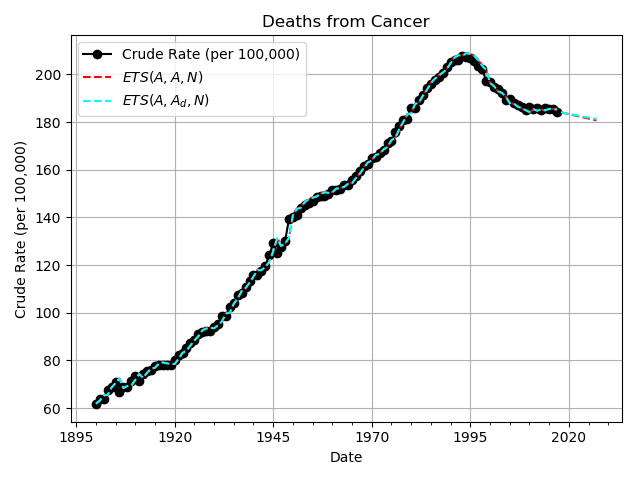
\includegraphics[width=0.5\textwidth]{results/US_ICD_LONGTERM_COMPARABLE_LEADING_Cancer_ets.png}
  \caption{Exponential smoothing functions $ETS(A,A*,N),\phi=0.98$ using Holt's linear trend method for \textit{Cancer} for the Longterm comparable leading causes of death for the United States}\label{fig:fig1}
\end{figure}

Scedasticity, forecast uncertainty, and cross-validation are not considered because it's not clear how to automate processing of such data to tune or choose models.

For each model, calculate AICc and choose the model $M(A(t_F))$ that has the lowest AICc. For example, see Table \ref{table:choosem}:

\begin{table}[H]
  \centering
  \begin{tabular}{lcc}
    \toprule
      $R_i(D(A))$       & AICc            & Predicted       \\
    \midrule
      $\bm{ETS(A,A,N)}$ & \textbf{128.37} & \textbf{180.73} \\
      $ETS(A,A_d,N)$    & 128.83          & 181.29          \\
    \bottomrule
  \end{tabular}
  \caption{Example AICc values of $R_i(D(A))$ for \textit{Cancer} for the Longterm comparable leading causes of death for the United States}
  \label{table:choosem}
\end{table}

Use each $M(A(t_F))$'s predicted value and generate all of the relative $B(t_F)$ values (setting negative values to 0) along with any scale functions based on the models (e.g. scaling by the relative prediction derivatives using $S_3$). For example, see Table \ref{table:btable}:

\begin{table}[H]
  \centering
  \begin{tabular}{lccc}
    \toprule
      Action  & $B(t_F)$ & $S_1$  & $S_3$  \\
    \midrule
      Name02  & 0.305    & 1      & 0.682  \\
      Name18  & 0.281    & 1      & 0.634  \\
      \ldots  & \ldots   & \ldots & \ldots \\
    \bottomrule
  \end{tabular}
  \caption{Example $B(t_F)$ values and model-based scale function values for the Longterm comparable leading causes of death for the United States}
  \label{table:btable}
\end{table}

Combine the table above with the manually calculated scale functions table \ref{table:scaletable} and any other calculated scale functions (e.g. $S_2(A_i)$) to create the final table with all scale function values. For example, see Table \ref{table:btablewithall}:

\begin{table}[H]
  \centering
  \begin{tabular}{lccccc}
    \toprule
      Action  & $B(t_F)$ & $S_1$  & $S_2$  & $S_3$  & $S_4$  \\
    \midrule
      Name02  & 0.305    & 1      & 0.386  & 0.682  & 1      \\
      Name18  & 0.281    & 1      & 0.435  & 0.634  & 1      \\
      \ldots  & \ldots   & \ldots & \ldots & \ldots & \ldots \\
    \bottomrule
  \end{tabular}
  \caption{Example $B(t_F)$ values with all scale function values for the Longterm comparable leading causes of death for the United States}
  \label{table:btablewithall}
\end{table}

Calculate the product of each action's $B(t_F)$ and its scale function values to produce the final $Z(t_F)$ table and then sort by the values in descending order and choose the top $k$ actions.

For the longterm comparable leading causes of death for the United States, the results\footnote{\texttt{python3 -m vbp.run modeled\char`_value\char`_based\char`_prioritization UCODUnitedStates --ets-no-multiplicative-models -k 5 -p 10 --manual-scales manual\char`_scale\char`_functions.xlsx --average-ages S2 --average-age-range 5}} are in Table \ref{table:ztable1} and Figure \ref{fig:k1}:

% US_ICD_LONGTERM_COMPARABLE_LEADING
\begin{table}[H]
  \centering
  \begin{tabular}{clc}
    \toprule
      $k$ & Action (Eliminate: \ldots) & $Z(t_F)$ \\
    \midrule
      1   & Name02 & 0.080375 \\
      2   & Name18 & 0.077476 \\
      3   & Name25 & 0.034373 \\
      4   & Name21 & 0.025423 \\
      5   & Name26 & 0.014776 \\
    \bottomrule
  \end{tabular}
  \caption{$Z(t_F)$ table for the Longterm comparable leading causes of death for the United States}
  \label{table:ztable1}
\end{table}

\begin{figure}[H]
  \centering
  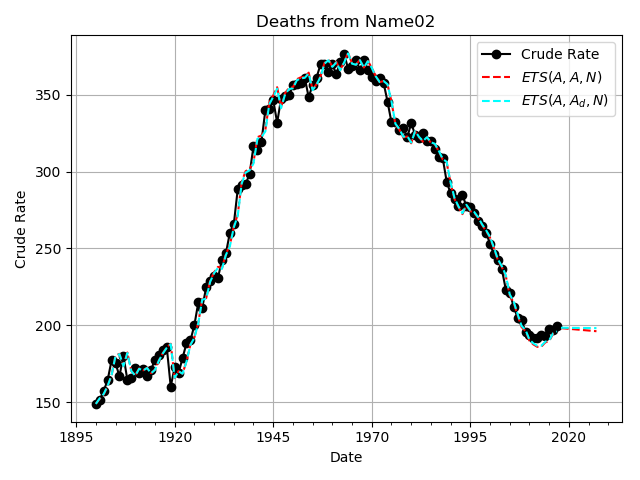
\includegraphics[width=0.5\textwidth]{results/US_ICD_LONGTERM_COMPARABLE_LEADING/Name02_ets.png}
  \caption{Highest priority action from the Longterm comparable leading causes of death for the United States: \textit{Name02}}\label{fig:k1}
\end{figure}

The same analysis is run on other mutually exclusive groupings of causes of death\footnote{Prefix the data source with the \texttt{-a} flag to run for all data types; for example: \texttt{python3 -m vbp.run modeled\char`_value\char`_based\char`_prioritization -a UCODUnitedStates \ldots}}:

\begin{enumerate}
  \vfill\eject
  % US_ICD_113_SELECTED_CAUSES_LEAVES
  \item ICD-9 and ICD-10 113 Cause List for the United States\cite{centers2017underlying}\textsuperscript{,}\footnote{Group Results By \enquote{Year} And By \enquote{ICD-10 113 Cause List}; Check \enquote{Export Results}; Uncheck \enquote{Show Totals}}\textsuperscript{,}\footnote{\scriptsize{\url{https://wonder.cdc.gov/wonder/help/ucd.html\#ICD-10\%20113\%20Cause\%20List}}}\textsuperscript{,}\footnote{\scriptsize{\url{https://www.cdc.gov/nchs/data/dvs/Multiple_Cause_Record_Layout_2016.pdf}, page 19; The list actually has 115 mututally exclusive groups instead of 113.}} in Table \ref{table:ztable2} and Figure \ref{fig:k2}:
    \begin{table}[H]
      \centering
      \begin{tabular}{clc}
        \toprule
          $k$ & Action (Eliminate: \ldots) & $Z(t_F)$ \\
        \midrule
          1   & Name029 & 0.042592 \\
          2   & Name029 & 0.038454 \\
          3   & Name056 & 0.028337 \\
          4   & Name072 & 0.021745 \\
          5   & Name025 & 0.019720 \\
        \bottomrule
      \end{tabular}
      \caption{$Z(t_F)$ table for the ICD-9 and ICD-10 113 Cause List for the United States}
      \label{table:ztable2}
    \end{table}
    \begin{figure}[H]
      \centering
      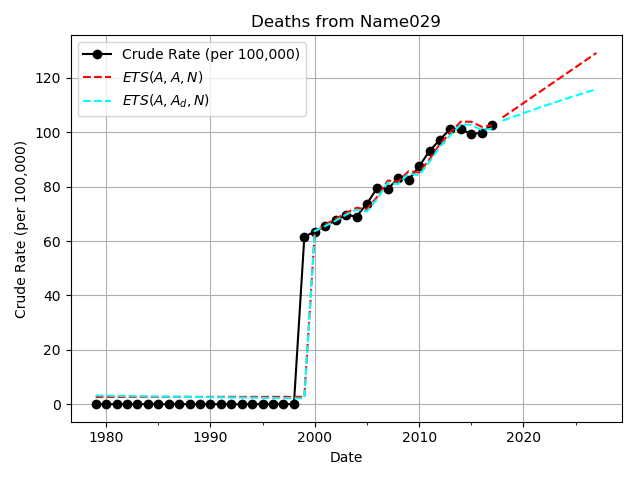
\includegraphics[width=0.5\textwidth]{results/US_ICD_113_SELECTED_CAUSES_LEAVES/Name029_ets.png}
      \caption{Highest priority action from the ICD-9 and ICD-10 113 Cause List for the United States: \textit{Name029}}\label{fig:k2}
    \end{figure}

  \vfill\eject
  % US_ICD_113_SELECTED_CAUSES_ALL
  \item ICD-9 and ICD-10 113 Cause List for the United States, including subtotals\cite{centers2017underlying}\textsuperscript{,}\footnote{Group Results By \enquote{Year} And By \enquote{ICD-10 113 Cause List}; Check \enquote{Export Results}; Uncheck \enquote{Show Totals}} in Table \ref{table:ztable2} and Figure \ref{fig:k2}:
    \begin{table}[H]
      \centering
      \begin{tabular}{clc}
        \toprule
          $k$ & Action (Eliminate: \ldots) & $Z(t_F)$ \\
        \midrule
          1   & Name048 & 0.049639 \\
          2   & Name009 & 0.031924 \\
          3   & Name082 & 0.021617 \\
          4   & Name082 & 0.019517 \\
          5   & Name111 & 0.019465 \\
        \bottomrule
      \end{tabular}
      \caption{$Z(t_F)$ table for the ICD-9 and ICD-10 113 Cause List for the United States, including subtotals}
      \label{table:ztable2}
    \end{table}
    \begin{figure}[H]
      \centering
      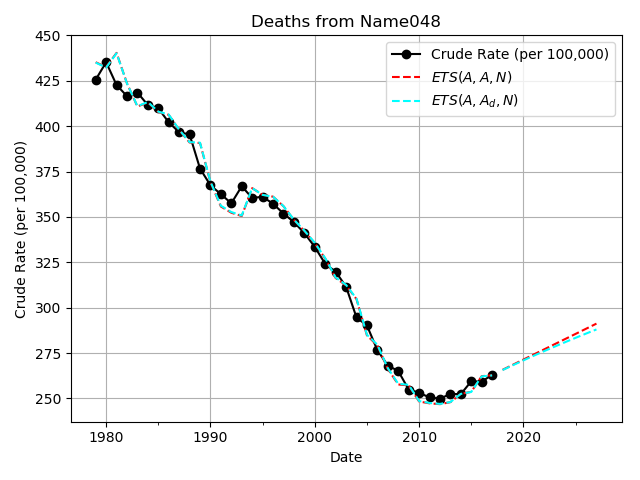
\includegraphics[width=0.5\textwidth]{results/US_ICD_113_SELECTED_CAUSES_ALL/Name048_ets.png}
      \caption{Highest priority action from the ICD-9 and ICD-10 113 Cause List for the United States, including subtotals: \textit{Name048}}\label{fig:k2}
    \end{figure}

  \vfill\eject
  % US_ICD_113_SELECTED_CAUSES_ROOTS
  \item ICD-9 and ICD-10 113 Cause List for the United States with only top-level groupings\cite{centers2017underlying}\textsuperscript{,}\footnote{Group Results By \enquote{Year} And By \enquote{ICD-10 113 Cause List}; Check \enquote{Export Results}; Uncheck \enquote{Show Totals}} in Table \ref{table:ztable3} and Figure \ref{fig:k3}:
    \begin{table}[H]
      \centering
      \begin{tabular}{clc}
        \toprule
          $k$ & Action (Eliminate: \ldots) & $Z(t_F)$ \\
        \midrule
          1   & Name01 & 0.113827 \\
          2   & Name27 & 0.049390 \\
          3   & Name27 & 0.044591 \\
          4   & Name51 & 0.044143 \\
          5   & Name05 & 0.039510 \\
        \bottomrule
      \end{tabular}
      \caption{$Z(t_F)$ table for the ICD-9 and ICD-10 113 Cause List for the United States with only top-level groupings}
      \label{table:ztable3}
    \end{table}
    \begin{figure}[H]
      \centering
      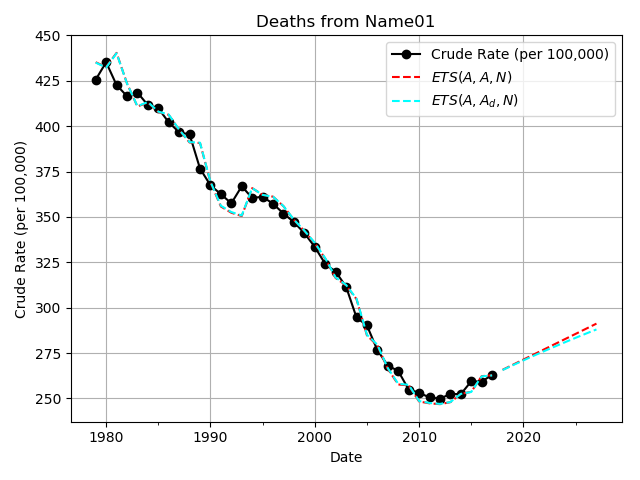
\includegraphics[width=0.5\textwidth]{results/US_ICD_113_SELECTED_CAUSES_ROOTS/Name01_ets.png}
      \caption{Highest priority action from the ICD-9 and ICD-10 113 Cause List for the United States with only top-level groupings: \textit{Name01}}\label{fig:k3}
    \end{figure}

  \vfill\eject
  % US_ICD10_CHAPTERS
  \item ICD-10 20 Chapters for the United States\cite{centers2017underlying}\textsuperscript{,}\footnote{Group Results By \enquote{Year} And By \enquote{ICD Chapter}; Check \enquote{Export Results}; Uncheck \enquote{Show Totals}} in Table \ref{table:ztable5} and Figure \ref{fig:k5}:
    \begin{table}[H]
      \centering
      \begin{tabular}{clc}
        \toprule
          $k$ & Action (Eliminate: \ldots) & $Z(t_F)$ \\
        \midrule
          1   & Name16 & 0.101677 \\
          2   & Name17 & 0.060121 \\
          3   & Name14 & 0.039507 \\
          4   & Name01 & 0.037175 \\
          5   & Name18 & 0.026494 \\
        \bottomrule
      \end{tabular}
      \caption{$Z(t_F)$ table for the ICD-10 20 Chapters for the United States}
      \label{table:ztable5}
    \end{table}
    \begin{figure}[H]
      \centering
      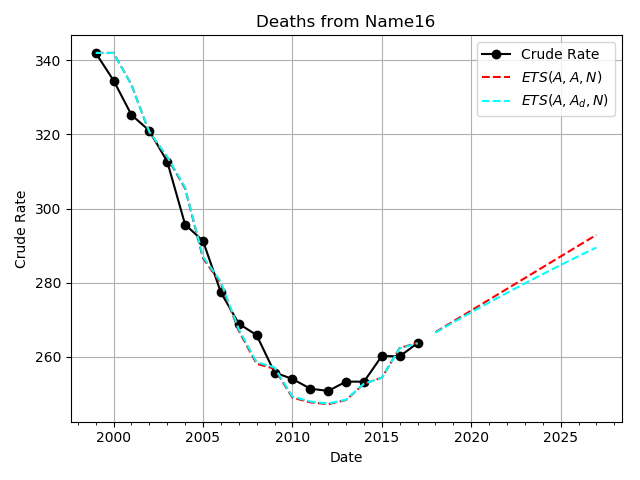
\includegraphics[width=0.5\textwidth]{results/US_ICD10_CHAPTERS/Name16_ets.png}
      \caption{Highest priority action from the ICD-10 20 Chapters for the United States: \textit{Name16}}\label{fig:k5}
    \end{figure}
  
  \vfill\eject
  % US_ICD10_SUB_CHAPTERS
  \item ICD-10 179 Sub-Chapters for the United States\cite{centers2017underlying}\textsuperscript{,}\footnote{Group Results By \enquote{Year} And By \enquote{ICD Sub-Chapter}; Check \enquote{Export Results}; Uncheck \enquote{Show Totals}} in Table \ref{table:ztable6} and Figure \ref{fig:k6}:
    \begin{table}[H]
      \centering
      \begin{tabular}{clc}
        \toprule
          $k$ & Action (Eliminate: \ldots) & $Z(t_F)$ \\
        \midrule
          1   & Name093 & 0.060440 \\
          2   & Name026 & 0.038374 \\
          3   & Name101 & 0.037231 \\
          4   & Name037 & 0.027645 \\
          5   & Name075 & 0.025999 \\
        \bottomrule
      \end{tabular}
      \caption{$Z(t_F)$ table for the ICD-10 179 Sub-Chapters for the United States}
      \label{table:ztable6}
    \end{table}
    \begin{figure}[H]
      \centering
      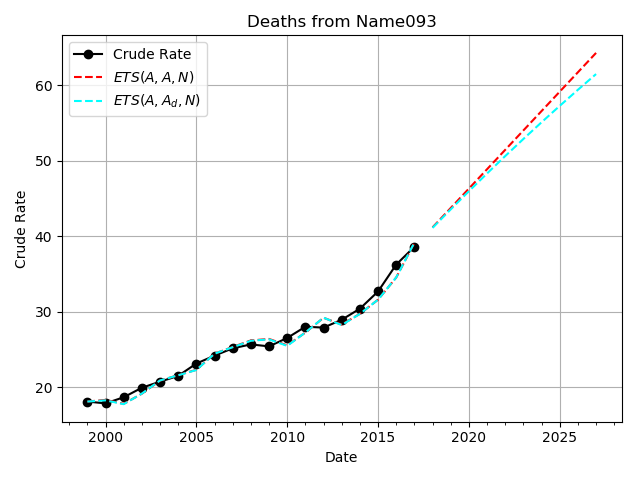
\includegraphics[width=0.5\textwidth]{results/US_ICD10_SUB_CHAPTERS/Name093_ets.png}
      \caption{Highest priority action from the ICD-10 179 Sub-Chapters for the United States: \textit{Name093}}\label{fig:k6}
    \end{figure}
    
  \vfill\eject
  % US_ICD10_MINIMALLY_GROUPED
  \item Minimally grouped (5,264) causes of death for the United States\cite{centers2017underlying}\textsuperscript{,}\footnote{Group Results By \enquote{Year} And By \enquote{Cause of death}; Check \enquote{Export Results}; Uncheck \enquote{Show Totals}}\textsuperscript{,}\footnote{Without $S_4$ due to the sheer number of causes.} in Table \ref{table:ztable7} and Figure \ref{fig:k7}:
    \begin{table}[H]
      \centering
      \begin{tabular}{clc}
        \toprule
          $k$ & Action (Eliminate: \ldots) & $Z(t_F)$ \\
        \midrule
          1   & Name0856 & 0.013730 \\
          2   & Name4563 & 0.012711 \\
          3   & Name2111 & 0.012563 \\
          4   & Name0653 & 0.011704 \\
          5   & Name3874 & 0.007563 \\
        \bottomrule
      \end{tabular}
      \caption{$Z(t_F)$ table for the Minimally grouped (5,264) causes of death for the United States}
      \label{table:ztable7}
    \end{table}
    \begin{figure}[H]
      \centering
      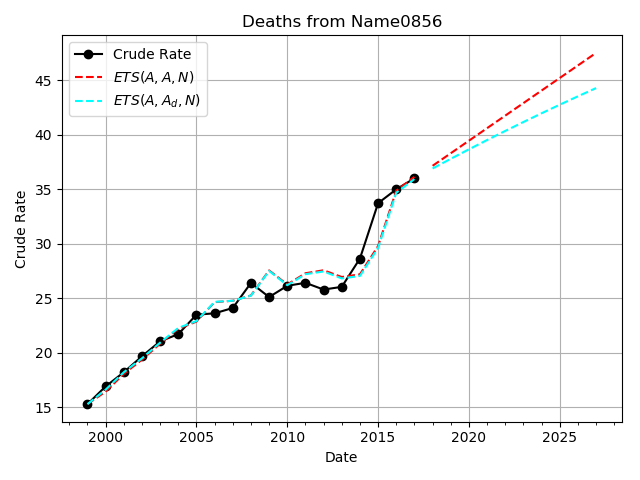
\includegraphics[width=0.5\textwidth]{results/US_ICD10_MINIMALLY_GROUPED/Name0856_ets.png}
      \caption{Highest priority action from the Minimally grouped (5,264) causes of death for the United States: \textit{Name0856}}\label{fig:k7}
    \end{figure}

  \vfill\eject
  % WORLD_ICD10_MINIMALLY_GROUPED
  \item Minimally grouped (11,316) causes of death for the World\cite{whomortality}\textsuperscript{,}\footnote{\label{no_s3}Without $S_3$ because comprehensive granular age data doesn't exist.}\textsuperscript{,}\footnote{Without $S_4$ due to the sheer number of causes.} in Table \ref{table:ztable8} and Figure \ref{fig:k8}:
    \begin{table}[H]
      \centering
      \begin{tabular}{clc}
        \toprule
          $k$ & Action (Eliminate: \ldots) & $Z(t_F)$ \\
        \midrule
          1   & Name01002 & 0.026866 \\
          2   & Name04954 & 0.024561 \\
          3   & Name05025 & 0.022585 \\
          4   & Name06345 & 0.019871 \\
          5   & Name01748 & 0.018749 \\
        \bottomrule
      \end{tabular}
      \caption{$Z(t_F)$ table for the Minimally grouped (11,316) causes of death for the World}
      \label{table:ztable8}
    \end{table}
    \begin{figure}[H]
      \centering
      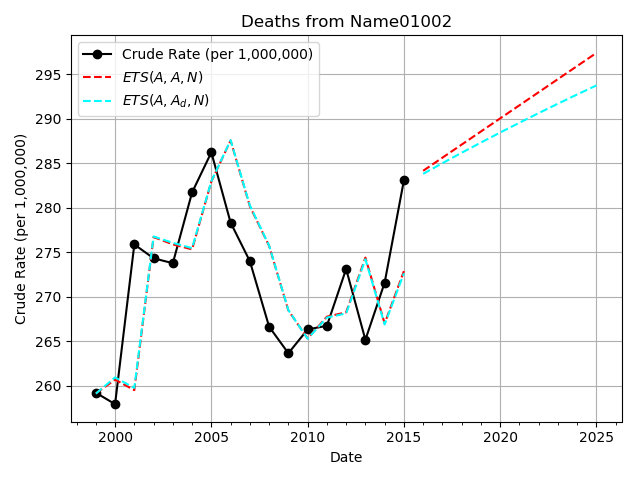
\includegraphics[width=0.5\textwidth]{results/WORLD_ICD10_MINIMALLY_GROUPED/Name01002_ets.png}
      \caption{Highest priority action from the Minimally grouped (11,316) causes of death for the World: \textit{Name01002}}\label{fig:k8}
    \end{figure}
  
  \vfill\eject
  % WORLD_ICD10_CHAPTERS_ALL
  \item ICD-10 22 Chapters for the World, including subtotals\cite{whomortality}\textsuperscript{,}\footnote{See footnote \ref{no_s3}.} in Table \ref{table:ztable9} and Figure \ref{fig:k9}:
    \begin{table}[H]
      \centering
      \begin{tabular}{clc}
        \toprule
          $k$ & Action (Eliminate: \ldots) & $Z(t_F)$ \\
        \midrule
          1   & Name038 & 0.160800 \\
          2   & Name216 & 0.097424 \\
          3   & Name059 & 0.092250 \\
          4   & Name151 & 0.046399 \\
          5   & Name148 & 0.034819 \\
        \bottomrule
      \end{tabular}
      \caption{$Z(t_F)$ table for the ICD-10 22 Chapters for the World, including subtotals}
      \label{table:ztable9}
    \end{table}
    \begin{figure}[H]
      \centering
      \includegraphics[width=0.5\textwidth]{results/WORLD_ICD10_CHAPTERS_ALL/Name038_ets.png}
      \caption{Highest priority action from the ICD-10 22 Chapters for the World, including subtotals: \textit{Name038}}\label{fig:k9}
    \end{figure}
  
  \vfill\eject
  % WORLD_ICD10_CHAPTER_ROOTS
  \item ICD-10 22 Chapters for the World with only top-level groupings\cite{whomortality}\textsuperscript{,}\footnote{See footnote \ref{no_s3}.} in Table \ref{table:ztable10} and Figure \ref{fig:k10}:
    \begin{table}[H]
      \centering
      \begin{tabular}{clc}
        \toprule
          $k$ & Action (Eliminate: \ldots) & $Z(t_F)$ \\
        \midrule
          1   & Name038 & 0.321104 \\
          2   & Name216 & 0.194456 \\
          3   & Name151 & 0.092581 \\
          4   & Name129 & 0.043816 \\
          5   & Name055 & 0.032951 \\
        \bottomrule
      \end{tabular}
      \caption{$Z(t_F)$ table for the ICD-10 22 Chapters for the World with only top-level groupings}
      \label{table:ztable10}
    \end{table}
    \begin{figure}[H]
      \centering
      \includegraphics[width=0.5\textwidth]{results/WORLD_ICD10_CHAPTER_ROOTS/Name038_ets.png}
      \caption{Highest priority action from the ICD-10 22 Chapters for the World with only top-level groupings: \textit{Name038}}\label{fig:k10}
    \end{figure}
  
  \vfill\eject
  % WORLD_ICD10_SUB_CHAPTERS
  \item ICD-10 211 Sub-Chapters for the World\cite{whomortality}\textsuperscript{,}\footnote{See footnote \ref{no_s3}.} in Table \ref{table:ztable11} and Figure \ref{fig:k11}:
    \begin{table}[H]
      \centering
      \begin{tabular}{clc}
        \toprule
          $k$ & Action (Eliminate: \ldots) & $Z(t_F)$ \\
        \midrule
          1   & Name059 & 0.216971 \\
          2   & Name148 & 0.076670 \\
          3   & Name197 & 0.038095 \\
          4   & Name189 & 0.032015 \\
          5   & Name092 & 0.031105 \\
        \bottomrule
      \end{tabular}
      \caption{$Z(t_F)$ table for the ICD-10 211 Sub-Chapters for the World}
      \label{table:ztable11}
    \end{table}
    \begin{figure}[H]
      \centering
      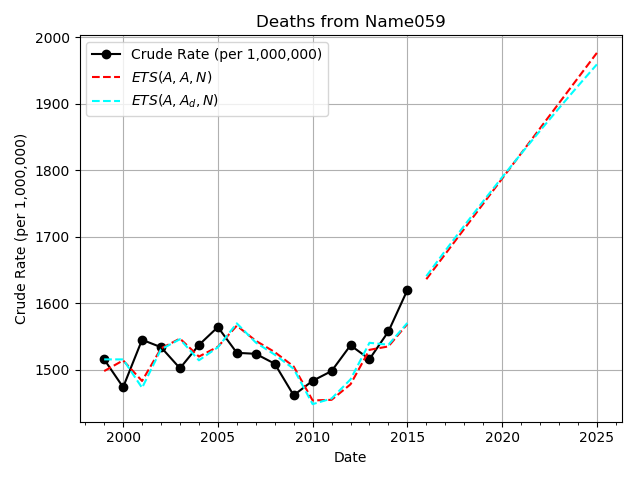
\includegraphics[width=0.5\textwidth]{results/WORLD_ICD10_SUB_CHAPTERS/Name059_ets.png}
      \caption{Highest priority action from the ICD-10 211 Sub-Chapters for the World: \textit{Name059}}\label{fig:k11}
    \end{figure}
\end{enumerate}

\section{Discussion}

TODO

% Column break before the Bibliography.
\vfill\eject

\bibliography{value_based_prioritization}

% Page break before the Appendix.
\newpage
\clearpage

\section{Appendix}

Notes on Section \ref{section-example}:

\begin{enumerate}
  \item \label{generateuslongterm} To generate the longterm comparable leading causes of death for the United States:
    \begin{enumerate}
      \item Generate data from 1959 for all long-term, comparable, leading causes of death\footnote{\scriptsize{\url{https://www.cdc.gov/nchs/data/dvs/lead1900_98.pdf}}}:
      
            \texttt{python3 -m vbp.run prepare\char`_data UCODUnitedStates}

      \item Rows 1900:1957 and the sheet \enquote{Comparability Ratios} in comparable\_ucod\_estimates.xlsx were manually input from \url{https://www.cdc.gov/nchs/data/dvs/lead1900_98.pdf}.
      \item Open comparable\_data\_since\_1959.xlsx and copy rows 1959:Present.
      \item Open comparable\_ucod\_estimates.xlsx and paste on top starting at 1959.
      \item Process comparable\_ucod\_estimates.xlsx with its \enquote{Comparability Ratios} sheet to generate comparable\_ucod\_estimates\_ratios\_applied.xlsx:
      
            \texttt{python3 -m vbp.run prepare\char`_data UCODUnitedStates --comparable-ratios}

    \end{enumerate}
  \item Age adjustment\footnote{\scriptsize{\url{https://seer.cancer.gov/seerstat/tutorials/aarates/definition.html}}} is not performed on crude rates because the goal of the example is to predict future \textit{relative} death rates which already implicitly takes into account population age changes over time.
  \item The WHO Mortality Database population and death statistics are quite incomplete, reporting only about $\frac{1}{3}$ of the world population and about $\frac{1}{3}$ of world deaths:
    \begin{figure}[H]
      \centering
      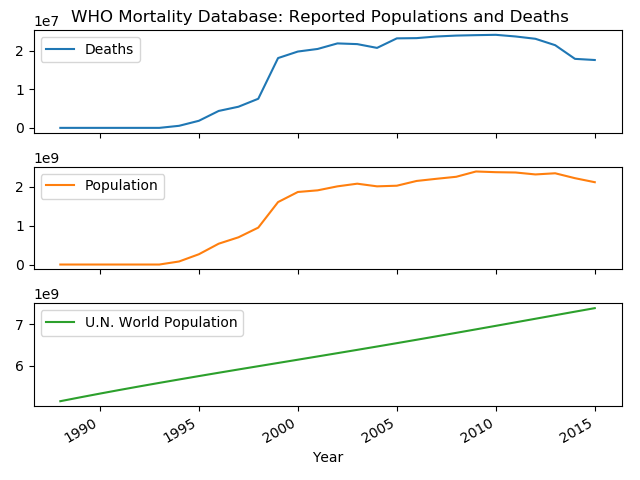
\includegraphics[width=0.5\textwidth]{results/who_mortality_db_population_deaths.png}
      \caption{WHO Mortality Database: Reported Population and Deaths}
    \end{figure}
  \item \enquote{Substantial research remains to develop robust and unbiased methods for measuring trends in case fatality rates, survival times, and disability due to specific causes, let alone collecting such data across all regions of the world. Despite these uncertainties, projections provide a useful perspective on population health trends and health policies, provided that they are interpreted with a degree of caution. Projections enable us to appreciate better the implications for health and health policy of currently observed trends, and the likely impact of fairly certain future trends, such as the ageing of the population, and the continuation of the epidemiological transition in developing countries.}\cite{mathers2006projections}
  \item \enquote{Accuracy in diagnosing causes of death still varies from one country to another. In addition the process of coding underlying causes of death involves some extent of misattribution or miscoding even in countries where causes are assigned by medically qualified staff. Main reasons are incorrect or systematic biases in diagnosis, incorrect or incomplete death certificates, misinterpretation of ICD rules for selection of the underlying cause, and variations in the use of coding categories for unknown and ill-defined causes.}\footnote{\scriptsize{\url{https://apps.who.int/healthinfo/statistics/mortality/whodpms/help/desc.htm}}}
\end{enumerate}

\end{document}

% Create PDF on Linux:
% FILE=value_based_prioritization; pkill -9 -f ${FILE} &>/dev/null; rm -f ${FILE}*aux ${FILE}*bbl ${FILE}*bib ${FILE}*blg ${FILE}*log ${FILE}*out ${FILE}*pdf &>/dev/null; pdflatex -halt-on-error ${FILE}; bibtex ${FILE} && pdflatex ${FILE} && pdflatex ${FILE} && (xdg-open ${FILE}.pdf &)
